\documentclass[a4paper, openany, 12pt]{article}

%% подключаем стандарт библиографии
\bibliographystyle{gost71u}

%% для "Abstract" в классе book
% \newenvironment{abstract}{}{}
% \usepackage{abstract}

%% подключаем преамбулу: в ней содержится подключение всех необходимых пакетов
\input{include/preambule.tex}

\begin{document}
    %% титульник
    \begin{center}
    %% *название института*
    \large\textbf{Министерство образования и науки Российской Федерации \\
    Московский физико-технический институт (государственный
    университет)} \\
    \vspace{1cm}

    %% *факультет/физтех-школа*
    Физтех-школа радиотехники и компьютерных технологий \\

    %% *название базовой кафедры и лаборатории*
    %% в случае ненадобности можно удалить
    Кафедра микропроцессорных технологий в интеллектуальных системах управления \\
    YADRO\\

    \vspace{3em}

    Выпускная квалификационная работа бакалавра
\end{center}

\begin{center}
    \vspace{\fill}
    %% *название вашей работы*
    \LARGE{Реализация в отладчике GDB поддержки вызова функций с векторным ABI для архитектуры RISC-V}

    \vspace{\fill}
\end{center}


\begin{flushright}
    \textbf{Автор:} \\
    Студент Б01-110 группы \\
    Радькин Кирилл Алексеевич \\
    \vspace{2em}
    \textbf{Научный руководитель:} \\
%%    *научная степень* \\
    Владимиров Константин Игоревич \\
    \vspace{2em}
%%    \textbf{Научный консультант:} \\
%%    *научная степень* \\
%%    Сергеев Сергей Сергеевич \\
\end{flushright}

\vspace{7em}

\begin{center}
    %% *лого*
    \includegraphics[width=100 pt]{MIPT_logo.jpg}\\
    Москва \the\year{}
\end{center}

%% выключаем отображение номера для этой страницы (титульник)
\thispagestyle{empty}

\newpage
\setcounter{page}{2}
\fancyfoot[c]{\thepage}
%% *надпись над верхним колонтинулом*
%% в случае ненадобности можно удалить
\fancyhead[L]{Реализация в отладчике GDB поддержки вызова функций с векторным ABI для архитектуры RISC-V}
\fancyhead[R]{}
    %% аннотация
    \fontsize{14}{21}\selectfont
    \begin{center}
	\textbf{Аннотация} \\[0.3 cm]
		Реализация в отладчике GDB поддержки вызова функций с векторным ABI для архитектуры RISC-V \\
		\textit{Радькин Кирилл Алексеевич} \\[1 cm]
	\end{center}

	; \\[1 cm]

	\newpage

	% \begin{center}
	%     \textbf{Abstract} \\[0.3 cm]
	%     Implementation in the GDB debugger of support for calling functions with a vector ABI for the RISC-V architecture \\
	%     \textit{Radkn Kirill Alekseevich} \\[1 cm]
	% \end{center}

	% ;
\newpage
    %% содержание
    \fontsize{14}{19}\selectfont
    \tableofcontents{}
    \newpage

    \fontsize{14}{21}\selectfont
    \section{Введение}
\label{sec:Intro} \index{Intro}

;

\newpage
 %% Введение
    \section{Постановка задачи}
\label{sec:Goal} \index{Goal}

Цель работы: реализовать в отладчике GDB для архитектуры RISC-V поддержку вызова функций,
использующих векторный ABI. Для выполнения данной цели были поставлены следующие задачи:

\begin{enumerate}
	\item Изучить генерацию отладочной информации для RISC-V компиляторами GCC и LLVM
	\item Реализовать RISC-V Vector Calling Convention в отладчике GDB
	\item Поддержать определение векторных типов и работу с ними в GDB
\end{enumerate}

\newpage
 %% Постановка задачи
    \section{Обзор архитектуры RISC-V}
\label{riscv} \index{riscv}

\subsection {Общая информация}
\label{riscv:general}

RISC-V -- это архитектура команд (ISA), основанная на принципах сокращённого
набора команд (RISC). Она была разработана в Калифорнийском университете в
Беркли в 2010 году и предназначена как для обучения, так и для промышленного
использования.

Одной из ключевых особенностей архитектуры является ее открытость. Спецификации
RISC-V находятся в открытом доступе. Архитектура свободна от лицензионных отчислений,
что позволяет использовать ее без юридических или финансовых ограничений.

Еще одним важным свойством архитектуры является ее модульность. Архитектура
состоит из базового набора целочисленных инструкций, который должен присутствовать
в любой реализации, и из дополнительных расширений, которые можно включать по
необходимости. Существует 4 варианта базового набора целочисленных
инструкций: \texttt{RV32I} и \texttt{RV64I}, которые описывают 32-разрядные или
64-разрядные адресные (далее разрядность будем называть \texttt{XLEN}, в терминах
спецификации RISC-V) пространства, и их подмножества, \texttt{RV32E} и \texttt{RV64E},
которые были добавлены для поддержки
небольших микроконтроллеров и обладающие вдвое меньшим набором целочисленных регистров.
Дополнительные расширения можно разделить на две группы: стандартные и пользовательские.
Среди стандартных дополнительных расширений можно выделить следующие:

\begin{itemize}
	\item \texttt{M} -- добавляет целочисленное умножение/деление
	\item \texttt{A} -- добавляет атомарные операции с памятью
	\item \texttt{F} -- добавляет регистры с плавающей точкой и соответствующие
	операции
	\item \texttt{D} -- добавляет регистры с плавающей точкой двойной точности и
	соответствующие операции
	\item \texttt{C} -- набор сжатых инструкций (с уменьшенной длиной)
	\item \texttt{V} -- векторные регистры и соответствующие операции
	\item \texttt{B} -- битовые операции
	\item \texttt{Zicsr} -- инструкции для работы с регистрами состояния и статуса
	ядра (Control and Status Registers, CSR)
	\item \texttt{Zifencei} -- инструкции для синхронизации потока инструкций и
	потока данных
\end{itemize}

Кроме того, существует аббревиатура G для обозначения базового набора расширений
\texttt{IMAFD\_Zicsr\_Zifencei}.

Архитектура поддерживается организацией RISC-V International, которая разрабатывает и
удтверждает стандартные расширения.

\subsection {Векторное расширение}
\label{riscv:rvv}

Векторное расширение (RISC-V Vector Extension, RVV) описывает набор инструкций и
регистров, предназначенных для эффективной параллельной обработки данных.

Каждое ядро, поддерживающее данное расширение, определяет два значения:

\begin{enumerate}
	\item ELEN -- максимальный размер векторного элемента (в битах),
	который может быть использован или создан векторной операцией.
	ELEN~$\geq 8$ и должно быть степенью 2.

	\item VLEN -- количество бит в одном векторном регистре.
	$2^{16} \geq$~VLEN~$\geq$~ELEN, и должно быть степенью 2.
\end{enumerate}

Векторное расширение добавляет 32 векторных регистра (\texttt{v0-v31}) и 7
непривилегированных CSR (\texttt{vstart, vxstat, vxrm, vcsr, vtype, vl, vlenb}).

\begin{itemize}
\item Регистр \texttt{vtype} является read-only CSR (т.~e. регистр, доступный только для
чтения) и может быть обновлен только с помощью специальных инструкций
\texttt{vset\{i\}vl\{i\}}.

Данный регистр хранит в себе следующую информацию:

\begin{itemize}
	\item Интерпретацию значений векторных регистров
	\item Способ группировки векторных регистров
	\item Способ обработки маскированных элементов
	\item Способ обработки элементов, длина которых превышает текущую длину вектора
\end{itemize}

\begin{figure}[H]
\centering
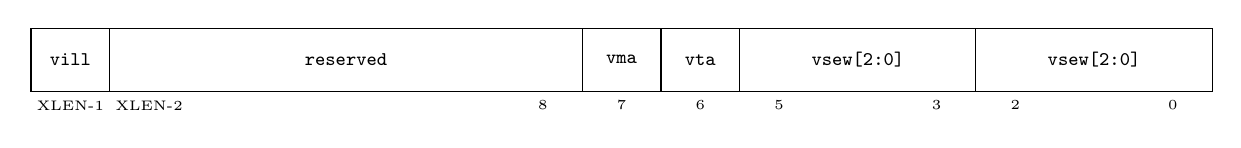
\begin{tikzpicture}
	\def\bitheight{0.4}

	\draw (0,0) rectangle (1, 2 * \bitheight);
	\node at (0.5, \bitheight) {\scriptsize \texttt{vill}};
	\node[below] at (0.5, 0) {\tiny XLEN-1};

	\draw (1,0) rectangle (7, 2 * \bitheight);
	\node at (4, \bitheight) {\scriptsize \texttt{reserved}};
	\node[below] at (1.5, 0) {\tiny XLEN-2};
	\node[below] at (6.5, 0) {\tiny 8};

	\draw (7,0) rectangle (8, 2 * \bitheight);
	\node at (7.5, \bitheight) {\scriptsize \texttt{vma}};
	\node[below] at (7.5, 0) {\tiny 7};

	\draw (8,0) rectangle (9, 2 * \bitheight);
	\node at (8.5, \bitheight) {\scriptsize \texttt{vta}};
	\node[below] at (8.5, 0) {\tiny 6};

	\draw (9,0) rectangle (12, 2 * \bitheight);
	\node at (10.5, \bitheight) {\scriptsize \texttt{vsew[2:0]}};
	\node[below] at (9.5, 0) {\tiny 5};
	\node[below] at (11.5, 0) {\tiny 3};

	\draw (12,0) rectangle (15, 2 * \bitheight);
	\node at (13.5, \bitheight) {\scriptsize \texttt{vsew[2:0]}};
	\node[below] at (12.5, 0) {\tiny 2};
	\node[below] at (14.5, 0) {\tiny 0};
\end{tikzpicture}
\caption{Поля регистра vtype}
\label{fig:vtype}
\end{figure}

\begin{itemize}
	\item \texttt{vill} -- флаг, указывающий на нелегальное значение
	\item \texttt{vma} -- если 0, то немаскированные элементы сохраняют свои значения
	после операций, если 1, то они могут как сохранить, так и быть переписаны единицами
	\item \texttt{vta} -- аналогично \texttt{vma}, только для элементов, которые
	находятся за текущей длиной вектора
	\item \texttt{vsew} -- текущее значение размера одного элемента (Selected Element
	Width, SEW)

	\begin{table}[h]
	\centering
	\begin{tabular}{|c|c|c|c|}
		\hline
		\multicolumn{3}{|c|}{vsew[2:0]} & SEW \\
		\hline
		0 & 0 & 0 & 8 \\
		\hline
		0 & 0 & 1 & 16 \\
		\hline
		0 & 1 & 0 & 32 \\
		\hline
		0 & 1 & 1 & 64 \\
		\hline
		1 & X & X & Reserved \\
		\hline
	\end{tabular}
	\caption{Соответствие между vsew[2:0] и SEW}
	\label{tab:vsew}
	\end{table}

	Значение SEW -- это размер в битах одного скалярного значения внутри векторного
	регистра.
	Соответственно, количество элементов в одном векторном регистре вычисляется как
	$\text{VLEN} / \text{SEW}$. В таблице~\ref{tab:sew} приведен пример для VLEN~=~128 бит.

	\begin{table}[H]
	\centering
	\begin{tabular}{|c|c|}
		\hline
		\texttt{SEW} & Количество элементов \\
		\hline
		8 & 16 \\
		\hline
		16 & 8 \\
		\hline
		32 & 4 \\
		\hline
		64 & 2 \\
		\hline
	\end{tabular}
	\caption{Пример для VLEN = 128 бит}
	\label{tab:sew}
	\end{table}

	\item \texttt{vlmul} -- текущее значение размера группы векторных регистров (Length
	Multiplier, LMUL)
\end{itemize}

Векторные регистры могут быть сгруппированы, чтобы одна векторная инструкция могла
оперировать сразу с несколькими векторными регистрами. Это повышает эффективность
обработки данных, позволяя работать сразу с несколькими регистрами (т.~е. с векторами
увеличенной длины). Значение LMUL представляет собой количество векторных регистров,
сгруппированных вместе.

Кроме того, LMUL может быть дробным значением. Дробное LMUL означает, что используется
только часть бит векторного регистра.

Таким образом, мы можем вычислить максимальное количество скалярных элементов, которыми
может оперировать одна векторная инструкция с текущими SEW и LMUL, как $\text{VLMAX} =
\text{LMUL} * \text{VLEN} / \text{SEW}$.

\item Регистр \texttt{vl} является read-only CSR и может быть обновлен только с помощью
специальных инструкций \texttt{vset\{i\}vl\{i\}}.

Данный регистр хранит в себе беззнаковое целочисленное значение, определяющее, с
каким количеством скалярных элементов будет взаимодействовать векторная инструкция.

\item Регистр \texttt{vlenb} является read-only CSR, который хранит в себе длину одного
векторного регистра в байтах, т.~е. $\text{VLEN} / 8$.

\end{itemize}

\subsection {Соглашение о вызовах}
\label{riscv:callconv}

Соглашение о вызовах (Calling Convention) -- набор правил, являющихся часть ABI (Application
Binary Interface), и определяющих особенности вызова функций. Этими правилами определяются
способы передачи аргументов функции и получения результата ее работы (через регистры процессора 
и/или через стек, порядок размещения аргументов), а также способы вызова и возврата из функций.
Далее в этом разделе я рассмотрю соглашение о вызовах для функций с векторными аргументами и
возвращаемыми значениями.

Для передачи векторных аргументов в функции существует несколько правил. Одно из таких правил
говорит, какие регистры должны использоваться для передачи аргументов и возвращаемого значения,
а какие регистры (точнее, их значения) должны быть сохранены между вызовами.
Регистр \texttt{v0} используется для передачи аргументов с типом векторной маски (т.~е. различные 
типы \texttt{vbool}) и для возвращаемого значения соответствующего типа. Регистры \texttt{v8}-\texttt{v23}
используются для передачи обычных векторных аргументов, кортежных векторных типов и оставшихся
аргументов с типом векторной маски. Эти же регистры используются для возвращаемого функцией
значения с одним из вышеуказанных типов.

Также, должно быть обеспечено сохранение значений регистров \texttt{v1}-\texttt{v7} и
\texttt{v24}-\texttt{v31}.

И последнее в списке, но не по важности, правило, по которому выбираются векторные регистры для
расположения на них аргументов. В первую очередь, мы должны выбрать некоторый последовательный
набор регистров, на котором может поместиться данный аргумент. Например, для типа \texttt{vint64m2\_t}
это может быть \texttt{v8}-\texttt{v9}, но не может быть \texttt{v8} и \texttt{v10}. Второй пункт
в данном правиле говорит о том, что номер первого регистра в данном наборе должен быть кратен значению
LMUL. Например, для типа \texttt{vint64m4\_t} это могут быть наборы \texttt{v8}-\texttt{v11} или
\texttt{v12}-\texttt{v15}, но не \texttt{v9}-\texttt{v12}.

Следует подчеркнуть, что поиск подходящего набора регистров каждый раз начинается с \texttt{v8},
следовательно, существует возможность, что номер первого векторного регистра из набора,
присвоенного векторному аргументу может быть меньше номера первого векторного регистра из набора,
присвоенного одному из предыдущих векторных аргументов. Например, для некоторой функции \texttt{void
foo (vint64m1\_t a, vint64m4\_t b, vint64m2\_t c)}, аргумент \texttt{a} будет располагаться на 
регистре \texttt{v8}, аргумент \texttt{b} на регистрах \texttt{v12}-\texttt{15}, а аргумент \texttt{c}
на регистрах \texttt{v10}-\texttt{v11}. 

\newpage
 %% Обзор архитектуры
    \section{Отладчик GDB}
\label{sec:gdb} \index{gdb}

\subsection {Основная информация}
\label{gdb:general}

GDB (GNU Project debugger) -- отладчик, программа, позволяющая анализировать и управлять
исполнением другой программы для нахождения ошибок в коде.
GDB поддерживает отладку программ, написанных на следующих языках:

\begin{itemize}
	\item Ada
	\item Assembly
	\item C/C++
	\item D
	\item Fortran
	\item Go
	\item Objective-C
	\item OpenCL
	\item Modula-2
	\item Pascal
	\item Rust
\end{itemize}

\subsection {Основные возможности}
\label{gdb:powers}

GDB позволяет запускать программы под своим управлением, анализировать и управлять их
исполнением.

Одна из основных возможностей это остановка исполнения программы в некоторой точке.
GDB позволяет установливать специальные метки в программе -- breakpoint-ы (точки останова),
которая указывает, в каком месте следует остановить выполнение программы. Breakpoint может
быть привязан как к строке в коде, так и к опредленному адресу. Во втором случае исполнение
программы будет остановлено перед исполнением инструкции, расположенной по указанному адресу.

После остановки программы, GDB позволяет выполнять множество различных операций,
полезных для поиска ошибок в коде.

Например, GBD позволяет просматривать значение переменных и изменять их. Для низкоуровневой
отладки существует аналогичная возможность отслеживания и редактирования значений определенных
регистров.

Следующей важной возможностью GDB является просмотр информации о текущем стековом фрейме и
стеке вызова функций.

Также, весьма полезной функцией является вызов отдельных функций программы.

\subsection {Отладочная информация: DWARF}
\label{gdb:debuginfo}

Отладочная информация -- данные, которые компилятор вставляет в исполняемые файлы. Эти
данные позволяются GBD понять, какие существуют переменные, функции, их местонахождение,
как соотносяться между собой машинные инструкции и исходный код и т.~д.

DWARF -- это соврменный формат отладочной информации, который используется в компиляторах GCC
и LLVM и поддерживается GDB.

Стандарт DWARF разработан так, чтобы быть применимым к множеству существующих языков, а также
иметь возможности к расширению для будущих языков.

\newpage
 %% GDB
    \section{Описание практической работы}
\label{sec:work} \index{work}

\subsection {Исправление генерации отладочной информации в компиляторе LLVM}
\label{work:clang_fix}

В процессе проведения различных экспериментов с генерацией отладочной информации,
было обнаружено, что для кортежных типов, таких как \texttt{vint8m4x2\_t}, компилятор LLVM
генерирует некорректную отладочную информацию о размере таких типов.
Компилятор не учитывал множитель \texttt{NFIELDS}.

Ниже приведена часть исходного кода LLVM с исправлением этой ошибки:

\begin{samepage}
\begin{lstlisting}[language=C++, caption=Исправление генерации информации о размере некоторых типов, label=lst:code:llvm_fix]
bool Fractional = false;
unsigned LMUL;
unsigned NFIELDS = Info.NumVectors;
unsigned FixedSize = ElementCount * SEW;
if (Info.ElementType == CGM.getContext().BoolTy) {
    // Mask type only occupies one vector register.
    LMUL = 1;
} else if (FixedSize < 64) {
    // In RVV scalable vector types, we encode 64 bits in the fixed part.
    Fractional = true;
    LMUL = 64 / FixedSize;
} else {
    LMUL = FixedSize / 64;
}

// Element count = (VLENB / SEW) x LMUL x NFIELDS
SmallVector<uint64_t, 12> Expr(
    // The DW_OP_bregx operation has two operands: a register which is
    // specified by an unsigned LEB128 number, followed by a signed LEB128
    // offset.
    {llvm::dwarf::DW_OP_bregx, // Read the contents of a register.
    4096 + 0xC22,             // RISC-V VLENB CSR register.
    0, // Offset for DW_OP_bregx. It is dummy here.
    llvm::dwarf::DW_OP_constu,
    SEW / 8, // SEW is in bits.
    llvm::dwarf::DW_OP_div, llvm::dwarf::DW_OP_constu, LMUL});
if (Fractional)
    Expr.push_back(llvm::dwarf::DW_OP_div);
else
    Expr.push_back(llvm::dwarf::DW_OP_mul);
// NFIELDS multiplier
if (NFIELDS > 1)
    Expr.append({llvm::dwarf::DW_OP_constu, NFIELDS, 
                 llvm::dwarf::DW_OP_mul});
// Element max index = count - 1
Expr.append({llvm::dwarf::DW_OP_constu, 1, 
             llvm::dwarf::DW_OP_minus});
\end{lstlisting}
\end{samepage}

Соответствующий патч с добавлением необходимого множителя \texttt{NFIELDS} был
мною предложен и принят в исходный код компилятора LLVM.

\subsection {Реализация в GDB}
\label{work:realisation}

Для того, чтобы поддержать RISC-V Vector Calling Convention в отладчике GDB, необходимо
было реализовать корректную передачу аргументов с векторными типами в функцию перед ее вызовом. 
Вторым требованием
является сохранение значений определенных регистров и их восстановление после окончание
исполнения функции, однако GDB самостоятельно сохраняет значения всех регистров перед вызовом
и восстанавливает их после, поэтому реализовывать данное требование не потребовалось.

Процесс размещения аргументов функции можно условно разделить на две стадии: определение корректного
местоположения аргументов функции в соответствии с ABI и размещение этих аргументов. В рамках
решения поставленных задач был модифицирован процесс установление правильного размещения
аргументов функции, добавлена поддержка определения правильного местоположения для векторных
аргументов.

Итак, в первую очередь, для определения векторного типа по его имени была написана следующая простая функция:

\begin{samepage}
\begin{lstlisting}[language=C++, caption=Функция для определения векторных типов, label=lst:func:is_rvv_type]
static bool
is_rvv_type (struct type *type)
{
  if (type)
  {
    if (type->name () && 
        (strncmp (type->name (), "__rvv", 5) == 0))
      return true;
    else if (type->code () == TYPE_CODE_TYPEDEF)
      return is_rvv_type (type->target_type ());
  }

  return false;
}
\end{lstlisting}
\end{samepage}

Например, тип \texttt{\_\_rvv\_int8m1\_t} (\texttt{vint8m1\_t}).

Для выбора способа передачи переменной векторного типа (через регистры или через память) была написана функция:

\begin{samepage}
\begin{lstlisting}[language=C++, caption=Функция для определения способа передачи значения аргумента, 
	           label=lst:func:riscv_call_arg_vector, breaklines=false]
static void
riscv_call_arg_vector (struct riscv_arg_info *ainfo,
                       struct riscv_call_info *cinfo,
                       struct type *func_arg_type)
{
  gdb_assert (((ainfo->length % cinfo->vlenb) == 0)
                || ainfo->length < cinfo->vlenb);

  if (!riscv_assign_vec_reg_location (ainfo, &cinfo->vector_regs,
                                      func_arg_type, cinfo->vlenb))
    {
      // Try to pass value by reference
      ainfo->argloc[0].loc_type = riscv_arg_info::location::by_ref;
      cinfo->memory.ref_offset = align_up (cinfo->memory.ref_offset, 
                                           ainfo->align);
      ainfo->argloc[0].loc_data.offset = cinfo->memory.ref_offset;
      cinfo->memory.ref_offset += ainfo->length;
      ainfo->argloc[0].c_length = ainfo->length;

      if (!riscv_assign_reg_location (&ainfo->argloc[1], 
                                      &cinfo->int_regs, 
                                      cinfo->xlen, 0))
        riscv_assign_stack_location (&ainfo->argloc[1], 
                                     &cinfo->memory,
                                     cinfo->xlen, cinfo->xlen);
    }
}
\end{lstlisting}
\end{samepage}

В первую очередь пытаемся разместить значение на векторных регистрах (в соответствии с RISC-V Vector
Calling Convention) с помощью функции \texttt{riscv\_assign\_vec\_reg\_location} (подробное описание
функции будет ниже). В случае неудачи, пытаемся передать значение по адресу, который, в свою очередь,
пытаемся сначала разместить на регистре общего назначения, используя  \texttt{riscv\_assign\_reg\_location}, 
или, на стеке, с помощью \texttt{riscv\_assign\_stack\_location}.

Реализация функции \texttt{riscv\_assign\_vec\_reg\_location}:

\begin{samepage}
\begin{lstlisting}[language=C++, caption=Функция для выбора набора регистров для передачи аргумента, 
			   label=lst:func:riscv_assign_vec_reg_location, breaklines=false]
static bool
riscv_assign_vec_reg_location (struct riscv_arg_info *ainfo,
                               struct riscv_vector_arg_reg *reg,
                               struct type *func_arg_type, int vlenb)
{
  /* Amount of data that is stored on one register */
  int data_length = vlenb;   
  
  struct riscv_arg_info::location *loc0 = &ainfo->argloc[0];
  struct riscv_arg_info::location *loc1 = &ainfo->argloc[1];
   
  const char *func_arg_type_name
    = (func_arg_type) ? func_arg_type->name () : nullptr;
   
  /* Try to get info about LMUL*/
  const char *lmul_pos = (func_arg_type_name) ? 
                          strstr (func_arg_type_name, "m") : nullptr;
  bool is_fractional_lmul = (lmul_pos && 
                             strncmp (lmul_pos, "mf", 2) == 0) ? 
                             true : false;
  int lmul = (lmul_pos) ? 
              ((is_fractional_lmul) ? 
                lmul_pos[2] - '0' : lmul_pos[1] - '0') : 1;
   
  /* If it is a segment type, it's name should ends with `xN_t`, 
     where N is * NFIELDS*/
  const char *nfields_pos = (func_arg_type_name) ? 
                          strstr (func_arg_type_name, "x") : nullptr;
  int nfields = (nfields_pos) ? nfields_pos[1] - '0' : 1;
   
  int num_required_regs = (ainfo->length <= vlenb) ? 
                           1 : ainfo->length / vlenb;
   
  if (is_fractional_lmul)
    {
      num_required_regs = nfields;
      data_length = data_length / lmul;
    }
   
  int first_regnum = -1;
   
  /* Representation of vector segmented types, like vint32m4x2_t,
      is different in Clang and GCC.
      In Clang, all types are arrays.
      In GCC, segmented types are struct's, 
      other vector types are arrays. */
  if (ainfo->type->code () == TYPE_CODE_ARRAY)
    {
      if (ainfo->type->target_type ()->code () == TYPE_CODE_BOOL)
        first_regnum = reg->try_use_v0 ();
      else
        first_regnum = reg->get_interval_start (num_required_regs, 
                                                nfields);
    }
  else if (ainfo->type->code () == TYPE_CODE_STRUCT)
    {
      first_regnum = reg->get_interval_start (num_required_regs, 
                                              nfields);
    }
   
  int last_regnum = first_regnum + num_required_regs - 1;
   
  if (first_regnum != -1)
    {
      loc0->loc_type = riscv_arg_info::location::in_several_regs;
      loc0->loc_data.regno = first_regnum;
      loc0->c_length = data_length;
      loc0->c_offset = 0;

      loc1->loc_type = riscv_arg_info::location::in_several_regs;
      loc1->loc_data.regno = last_regnum;
      loc1->c_length = 0;
      loc1->c_offset = 0;
   
      return true;
    }
   
  return false;
}
\end{lstlisting}
\end{samepage}

В данной функции мы сначала определяем параметры LMUL и NFIELDS. К сожалению, эти параметры
пока невозможно получить более \enquote{чистым} способом -- из отладочной информации, т.~к. их там
попросту нет. Мы обладаем только информацией о размере типа, из которой мы можем сделать
вывод о количестве необходимых векторных регистров, но не о множителе LMUL, необходимом
для корректной реализации векторного соглашения о вызовах.
Далее, вызывая
метод \texttt{get\_interval\_start} у объекта \texttt{struct riscv\_vector\_arg\_reg *reg},
который сохраняет в себе информацию об уже занятых регистрах, мы получаем номер первого
регистра в наборе (и вычисляем номер последнего регистра), в котором будет сохранено 
необходимое значение.

Как было сказано выше, для сохранения информации об уже занятых регистрах, была
написана структура данных \texttt{riscv\_vector\_arg\_reg}:

\begin{samepage}
\begin{lstlisting}[language=C++, caption=Структура для хранения информации о свободных векторных регистрах, 
			label=lst:struct:riscv_vector_arg_reg, breaklines=false]
struct riscv_vector_arg_reg_interval
{
  int first;
  int last;
};

struct riscv_vector_arg_reg
{
  riscv_vector_arg_reg (int first, int last)
      : available_intervals{ { first, last } }
  {
    /* Nothing. */
  }

  int
  get_interval_start (int count, int NFIELDS = 1)
  {
    gdb_assert (count % NFIELDS == 0);

    int LMUL = count / NFIELDS;
    for (auto cur_interval = available_intervals.begin ();
         cur_interval != available_intervals.end (); ++cur_interval)
      {
        int cur_first = cur_interval->first;
        int cur_last = cur_interval->last;
        if ((cur_first - RISCV_V0_REGNUM) % LMUL != 0) 
             /* According to RISC-V Vector ABI,
             first register number should be
             a multiple of LMUL */
          {
            cur_first -= (cur_first - RISCV_V0_REGNUM) % LMUL;
            cur_first += LMUL;
          }

        if ((cur_last - cur_first + 1) >= count)
          {
          if (cur_first > cur_interval->first)
            {
              available_intervals.insert 
                (cur_interval, { cur_interval->first, cur_first - 1 });
            }

            cur_interval->first = cur_first + count;

            return cur_first;
	  }
      }

    return -1;
  }

  int
  try_use_v0 ()
  {
    if (is_v0_used)
      return get_interval_start (1);
    else
      {
        is_v0_used = true;
        return RISCV_V0_REGNUM;
      }
  }

  bool is_v0_used
      = false; /* To pass masks we should use v0, if it's available */

  std::list<riscv_vector_arg_reg_interval> available_intervals;
};
\end{lstlisting}
\end{samepage}

Данные о незанятых векторных регистров хранятся в виде интервалов вида 
\texttt{\{first, last\}} с номерами регистров. В случае, если нам необходимо
выделить какой-то набор регистров, лежащий в интервале, этот интервал
разбивается на 3 части: необходимый нам набор, интервал до и интервал после
необходимого набора. Эти новые интервалы сохраняются взамен старого интервала\
(в случае, если они не являются пустыми).

Кроме того, отдельно отслеживается занятость регистра \texttt{v0}, т.~к. он
используется для передачи векторных масок.

Последняя важная часть, это обработка введенного варианта расположения
переменной на регистре \texttt{riscv\_arg\_info::location::in\_several\_regs}
в функции \texttt{riscv\_push\_dummy\_call}:

\begin{samepage}
\begin{lstlisting}[language=C++, caption=Запись необходимого значения в соответствующие регистры в кэше, 
		label=lst:switch:in_several_regs, breaklines=false]
case riscv_arg_info::location::in_several_regs:
{
  const gdb_byte *cur_contents = info->contents;
  int cur_c_length = info->argloc[0].c_length;
  for (int cur_regno = info->argloc[0].loc_data.regno;
       cur_regno <= info->argloc[1].loc_data.regno; cur_regno++)
    {
      riscv_regcache_cooked_write (cur_regno, cur_contents,
                                   cur_c_length, regcache,
                                   call_info.flen);
      cur_contents += cur_c_length;
    }

  second_arg_length = 0;
}
\end{lstlisting}
\end{samepage}







\newpage %% GDB

    %% НЕ ТРОГАЙТЕ!!!
    \nocite{*}
    \bibliography{references}

    %% в зависимости от надобности подключаем раздел "Приложение"
    % \newpage
    % \input{Appendix.tex}
\end{document}